\documentclass{sig-alternate}
\usepackage{tabularx}
\usepackage[noabbrev]{cleveref}
\usepackage{times}

\begin{document}

% Copyright
\setcopyright{acmcopyright}
%\setcopyright{acmlicensed}
%\setcopyright{rightsretained}
%\setcopyright{usgov}
%\setcopyright{usgovmixed}
%\setcopyright{cagov}
%\setcopyright{cagovmixed}


% DOI
%\doi{10.475/123_4}

% ISBN
%\isbn{123-4567-24-567/08/06}

%Conference
%\conferenceinfo{PLDI '13}{June 16--19, 2013, Seattle, WA, USA}

%\acmPrice{\$15.00}

%
% --- Author Metadata here ---
\conferenceinfo{MSR}{'16 Austin, Texas USA}
% --- End of Author Metadata ---

\title{The evolution of GHTorrent: growing an open access dataset 10x}
\numberofauthors{1} %  in this sample file, there are a *total*
% of EIGHT authors. SIX appear on the 'first-page' (for formatting
% reasons) and the remaining two appear in the \additionalauthors section.
%
\author{
% The command \alignauthor (no curly braces needed) should
% precede each author name, affiliation/snail-mail address and
% e-mail address. Additionally, tag each line of
% affiliation/address with \affaddr, and tag the
% e-mail address with \email.
%
% 1st. author
\alignauthor Georgios Gousios\\
       \affaddr{Radboud University Nijmegen}\\
       \affaddr{Nijmegen, the Netherlands}\\
       \email{g.gousios@cs.ru.nl}
}

\maketitle
\begin{abstract}

With over 31 million repositories and 12 million users, GitHub is by far the
biggest open source forge in existense. Since early 2012, the GHTorrent project
has been retrieving data from GitHub's open access API and offering them to the
repository mining community.  In this paper, we describe how we grew GHTorrent
to 10x the size of early 2013, while at the same time improving its coverage,
quality and versatility and offering data access services to hundrends of
researchers.

\end{abstract}

%
% The code below should be generated by the tool at
% http://dl.acm.org/ccs.cfm
% Please copy and paste the code instead of the example below. 
%
\begin{CCSXML}
<ccs2012>
 <concept>
  <concept_id>10010520.10010553.10010562</concept_id>
  <concept_desc>Computer systems organization~Embedded systems</concept_desc>
  <concept_significance>500</concept_significance>
 </concept>
 <concept>
  <concept_id>10010520.10010575.10010755</concept_id>
  <concept_desc>Computer systems organization~Redundancy</concept_desc>
  <concept_significance>300</concept_significance>
 </concept>
 <concept>
  <concept_id>10010520.10010553.10010554</concept_id>
  <concept_desc>Computer systems organization~Robotics</concept_desc>
  <concept_significance>100</concept_significance>
 </concept>
 <concept>
  <concept_id>10003033.10003083.10003095</concept_id>
  <concept_desc>Networks~Network reliability</concept_desc>
  <concept_significance>100</concept_significance>
 </concept>
</ccs2012>
\end{CCSXML}

\ccsdesc[500]{Computer systems organization~Embedded systems}
\ccsdesc[300]{Computer systems organization~Redundancy}
\ccsdesc{Computer systems organization~Robotics}
\ccsdesc[100]{Networks~Network reliability}


%
%  Use this command to print the description
%
\printccsdesc

\keywords{ACM proceedings; \LaTeX; text tagging}

\section{Introduction}


\section{Current status}

\begin{table}
  \centering
  \begin{small}
  \label{tab:datasetsize}
  \begin{tabular}{llll}
    \hline
    \bfseries{Entity} & \bfseries{MongoDB} & \bfseries{MySQL} & \bfseries{Diff to 2013} \\
    \hline
      Events                     & 476,047,453 & ---           & 11.1x\\
      Users                      & 6,733,244   & 9,277,113     & 8.4x \\
      \ldots of which fake       & ---         & 2,435,859     & ---\\
      \ldots of which deleted    & ---         & 271,590       & ---\\
      \ldots of which geolocated & ---         & 1,108,784     & \\
      Repositories               & 28,851,321  & 25,578,419    & 21.8x\\
      \ldots of which forks      & ---         & 10,486,114    & --- \\
      \ldots of which deleted    & ---         & 4,986,095     & ---\\
      Commits                    & 367,815,284 & 362,057,838   & 12.3x \\
      Issues                     & 24,165,582  & 25,351,996    & 10.3x \\
      Pull requests              & 11,944,969  & 11,114,625    & 9.7x \\
      Issue comments             & 42,021,374  & 43,416,372    & 14.6x\\
      Watchers (stars)           & 51,698,373  & 37,022,681    & 6.6x\\
      \hline
  \end{tabular}
    \caption{GHTorrent database contents as of Jan 14, 2016. The difference column reports the difference to the numbers reported in reference ~\cite{Gousi13}.}
  \end{small}
\end{table}

\subsection{Three operating modes}

GHTorrent primarily focuses on following GitHub's event stream and, by applying
dependency-based recursive retrieval, to retrieve all linked entities (e.g.  all
committers, commit contents, repository etc for a single PushEvent).
Through the years, we discovered that this mode of operation, while efficient,
has three issues: i) in case of failures (which are frequent, see
Figure~\ref{fig:service-stats}), the resulting data is inconsistent,
ii) we cannot update volatile information about users and projects (e.g. user
locations) as GitHub does not emit any related events, and
iii) we cannot collect all the data for projects that existed before GHTorrent
For those reasons, we introduced two additional operating modes:

\begin{description}

  \item[Full-repo / user retrievals] When an error is reported by a GHTorrent
    user for a specific repository or a collection of repositories, we run a
    process that will retrieve all information about a given user or repository
    recursively. The same process has been used by several OSS projects to
    generate community analytics; the
    GHTorrent-Vagrant\footnote{https://github.com/ghtorrent/ghtorrent-vagrant}
    project was thus created to streamline the installation of GHTorrent for
    such purposes.

  \item[Bi-monthly update] For each non-deleted repository and user in the
    database, GHTorrent retrieves a fresh copy of its entry on GitHub. This way,
    GHTorrent can mark projects and users as deleted (they exist in GHTorrent
    but not on GitHub) and can update their metadata (e.g. programming
    languages).

\end{description}

Furthermore, to eliminate data retrieval holes caused by arbitrary errors in
collecting the event stream, we synchronize the contents of the event collection
with Github Archive~\footnote{https://www.githubarchive.org} daily.


\begin{figure}
  \begin{center}
    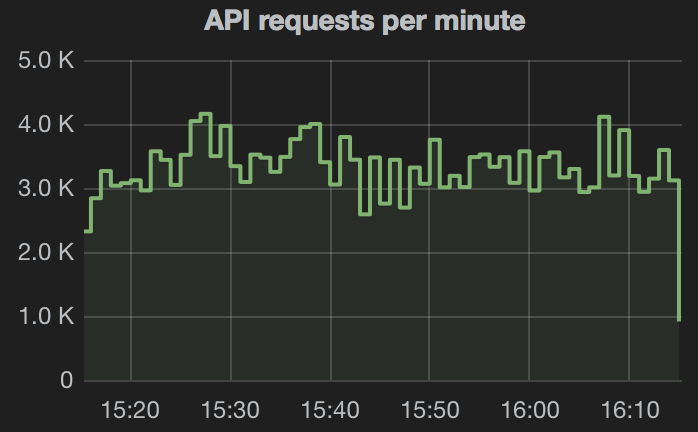
\includegraphics[scale=0.332]{api-requests}
    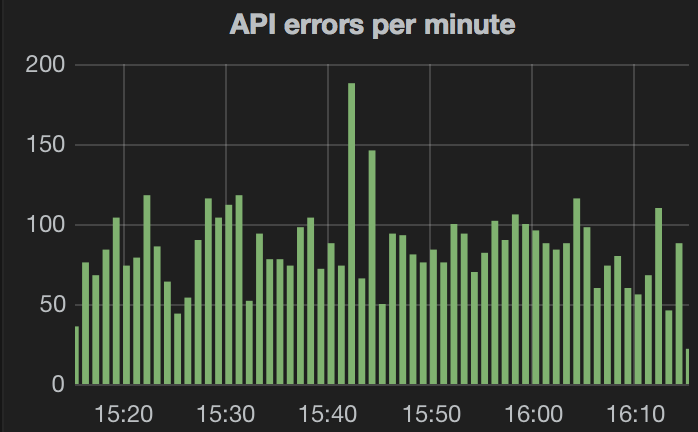
\includegraphics[scale=0.332]{api-errors}
    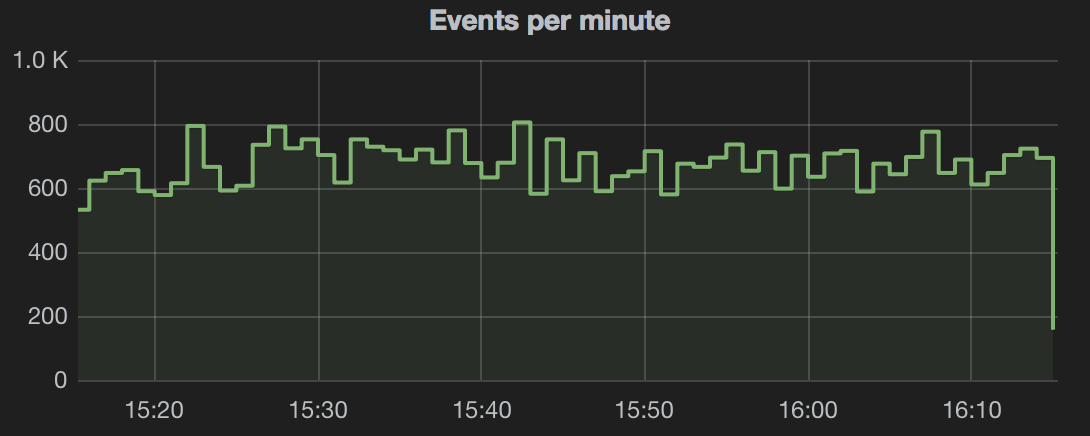
\includegraphics[scale=0.438]{events-per-min}
  \end{center}
  \caption{Service monitoring graphs for a typical day (Jan 18, 2016)}
  \label{fig:service-stats}
\end{figure}

\subsection{Better Repository Descriptions}


\subsection{Repository Languages}
GitHub by default calculates programming language usage statistics for all
repositories. Upon visiting a repository, the user can view this information
like so:

\noindent
\includegraphics[scale=0.243]{languages}

Until recently (Feb 2015), this information was not available through the API
and thus researchers could only rely on the main repository language when
selecting repositories for analysis. This led to sub-optimal repository
selections, e.g. in the, very frequent, case where the primary and the secondary
language are the same. As of Nov 2015, GHTorrent collects size information (in
bytes) for all programming languages in all repositories; this information is
timestamped at the moment the retrieval was done. With it, researchers can
refine the selection of repositories, cluster repositories in interesting ways
(e.g. those that contain Javascript and HTML are probably web projects) and even
monitor the evolution of programming language use.

\subsection{Forks}

When a project is forked, GitHub will create an identical copy of the project
repository and initialize a new issue tracker for it. Internally, the repository
contents are not really duplicated; GitHub will use a copy-on-write
mechanism to minimize disk space use.\footnote{http://githubengineering.com/counting-objects/} This process makes forking very cheap for GitHub.

When GHTorrent encounters a fork event, it treats the fork as a new repository.
It thus recursively retrieves all information about the fork, such as the
repository owner and issue labels. In the early versions of
GHTorrent, recursive retrieval also included commits. For big and popular
projects, such as Ruby on Rails (55k commits, 11k forks),
this process required several (thousand) additional GitHub API calls, which
quickly depleted GHTorrent limited API rates. For this reason, GHTorrent implemented a mechanism that only retrieve new commits from forks until
it found a shared commit with the parent repository; it would then switch
to copying commits internally within the GHTorrent database. This trick worked
with formidable efficiency, as it cut down on API calls (and the time required
to process them) by more than 95\% for big projects.

However, its very efficiency caused a new problem; \emph{too many} forks where
processed meant that the table that records the association between commits and
repositories (\texttt{project\_\-commits}) grew uncontrollably. Just for Ruby on
Rails, this table would store more than 500M rows. The root of the problem
is that \texttt{project\_commits} models an $M \times N$ relationship between
projects and commits and this cannot be normalized further without signicant
duplication (Boyce-Codd Normal form).

Concequently, retrieving fork commits was converted to an optional
configuration parameter and are not retrieved by default. Therefore, the
(\texttt{project\_\-commits}) table is inconsistent with respect to
fork commits.

\subsection{Better User Identification}

When a commit is being processed by GHTorrent, a user must be associated with it.
GHTorrent first attempts to query GitHub for information about the committer
and, if this fails (the committer is not registered with GitHub), then it
creates a fake user to register this commit with. Until recently, it was not
possible to identify fake users; GHTorrent now marks them as such in the MySQL
database. Moreover, it can convert fake users to normal users if a user with
the provided email is registered with GitHub in the future.

Moreover, similarly to projects, users can also delete their accounts.
GHTorrent keeps track of deleted users by marking them as such. This helps
researchers to eliminate inactive users from their analyses.

\subsection{User Geolocation}

Almost 1.3M GitHub users share their location in their profiles. GHTorrent uses
this information to \emph{geolocate} those users. Geolocation refers to the
process of converting a text string potentially indicating the address of a
place on earth to the longitude and latitude co-ordinates corresponding to this
address. As GitHub's address field is free-form text, there are no guarantees
about the format of the address fields. GHTorrent uses the OpenStreetMap
geolocation service (Nominatim) for this functionality. To overcome Nomitatim's
API restrictions, it caches geolocated places in the Mongo database. 160,000
cached addresses have been collected so far, with a very high cache hit ratio.
An example application of geolocation information can be seen in
Figure~\ref{fig:dev-map}.

It is important to notice that geolocation in GHTorrent is a best effort
approach. Initially, not all user provided location strings can be decoded to a
real address; on the one hand, several users provide fictional addresses while
on the other the Nominatim service is not top of the crop for geolocation.
Moreover, users may choose not to share their addresses while cultural
differences in online privacy perceptions may lead to whole clusters of users
being under-represented. Consequently, care must be applied when drawing
conclusions from this data.

\begin{figure}
  \begin{center}
    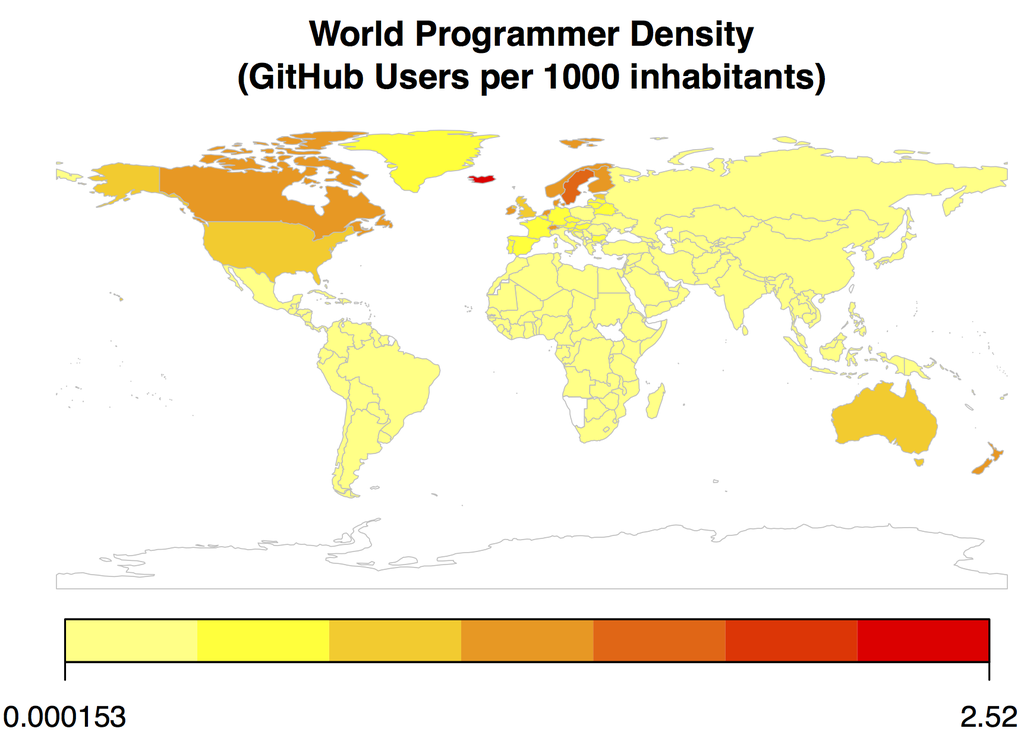
\includegraphics[scale=0.2]{dev-map.png}
  \end{center}
  \caption{GHTorrent users that registered a location plotted on a map after
  geocoding them.}
  \label{fig:dev-map}
\end{figure}

\subsection{Discontinued and Incomplete}

The following services/features have been discontinued:

\begin{description}

  \item[Organization Members and Collaborators] On Nov 2014, GitHub disabled
    the repository membership query end point. Interestingly, they did not
    disable the membership events. As GHTorrent follows the event stream,
    it can retrieve new repository members, but it will not remove 

  \item[Followers] 

  \item[Lean GHTorrent] Lean GHTorrent~\cite{GVSZ14} was effectively a dataset
    slicer, for users that could not use the dataset in its entirety. Through 2
    years of operation, Lean GHTorrent only received 55 user requests, while to
    the best of our knowledge no work resulted from its use. Since January 2016,
    Lean GHTorrent was discontinued.

\end{description}

\subsection{Azure and Data Lake}

GHTorrent's data collection process was recently moved to the Azure cloud
platform. The move to Azure was necessitated for two reasons: i) to ensure the
sustainability of GHTorrent in the face of growing hardware requirements ii) to
better allocate available developer resources to the future of GHTorrent. The
move was motivated by a donation of free Azure usage credits.

The move to Azure has the following benefits for the research community:

\begin{itemize}

  \item GHTorrent servers are now more capable of dealing with the accumulated
    data sizes and Github growth. This means more accurate data collection
    and more frequent retrospective updates.

  \item The online dataset access services will run on more powerful servers,
    leading to better query performance and access to real-time replicas of
    the main project databases.

  \item The dataset and collection process will be integrated with Azure
    Data Lake, a big data processing platform featuring a common backend
    and multiple front ends. Researchers will be soon able to use state
    of the art big data analysis tools (e.g. {\sc usql}, Spark) to scale
    research across all GHTorrent data in real-time.

\end{itemize}


\subsection{Service updates}

The following changes took place in the 

Weekly MySQL dumps, daily mongoDb dumps

Mongo, MySQL, Juniper setup with MySQL/Mongo

\section{Lessons learned}



\section{Open research topics}

Due to the availability and homogeneity of data, GitHub has been the target of
hundreds of researchers. GHTorrent has been in the epicentre of several research
efforts; we estimate that close to 80 papers have been written using data from
GHTorrent.\footnote{GHTorrent's ``Hall of fame'' page lists at least 20:
http://ghtorrent.org/halloffame.html} With GHTorrent data, schemata and
limitations being understood by a large number of software engineering
researchers, new capabilities on offer and a large scale data analysis
infrastructure in place, the research community can collaborate to answer deeper
questions and impact the practice of millions of developers per day.

To 

\begin{description}

  \item[Developer clustering] Looking at technology used, interaction types, geographies, social circles…
    Identify different community structures.  Eg., to better understand the community dynamics

    Are there clusterings of languages that developers use together


  \item[Project clustering]

    You want to compare across similar projects or project types that do not matter, e.g. student projects. Features of gihub might also matter for different types. Monitor these indicators.
Expectations on github projects, download only, contributions, advertising, using the tools only, …


  \item[Developer productivity] Drive-by contributions: Is the gain in sustained contribution from fewer people or smaller individual contributions from many people

  What teams, projects are more productive, what are their practices and patterns?

Tools for hiring decision managers on developers and their code


  \item[Community best practices]

understand characteristics of successful projects, tell how our projects are doing and to determine if someone else’s project is solid enough to depend on or worthy of investment

What is the correlation/interaction between the typical SE and community metrics

Identify different community structures.  Eg., to better understand the community dynamics

Timelines, engagement, diversity, .. Both to support decisions to use projects from others as well as quality of our projects

Contributor evolution: What are the stages and what are the activities to drive people further along the engagement funnel


  \item[Cross-project code analysis]
Are there clusterings of languages that developers use together

Files contributed by many distinct developers tend to be more buggy.  Could we create a tool using the github data

Cross-project API analysis



  \item[Trends and outliers]
4 labels: inactive, active, hyper-active…, comparing MS to Google or Facebook repos


Technology, language, projects, etc being used.  How to predict trends

Clustering different repros yielded some extreme outliers that had to be filtered out to have a meaningful results.  This data gives us opportunity to look for these anomalous activity.

Language popularity

  \item[Operationalization of research] Maintaining process and policy

\end{description}

\section{Conclusions}



\section*{Acknowledgements}

The GHTorrent project would like to thank Microsoft for their generous support
that enabled the move to the Azure cloud. The author would also like the
numerous GHTorrent users (Bogdan Vasilescu and Daniel German require special
mention) for the fruitful discussions that led to a better GHTorrent for
everybody.

\bibliographystyle{acm}
\bibliography{ghtorrent-update}


\end{document}
